% !TeX root = ./test.tex
% !TEX program = xelatex

\documentclass[topmenu]{taltechslides}

% DEFINE HOW TOC IS DISPLAYED
\AtBeginSection[]
{
\begin{frame}<beamer>
    % \frametitle{Outline}
    \begin{columns}[t]
        \begin{column}{.5\textwidth}
            \tableofcontents[currentsection, hideothersubsections, sections={1-3}]
        \end{column}
        \begin{column}{.5\textwidth}
            \tableofcontents[currentsection, hideothersubsections, sections={4-6}]
        \end{column}
    \end{columns}
\end{frame}
}

\begin{document}

% MAKE THE TITLE PAGE
\maketitle

% START NEW PART (optional?)
\part{Main}

% START NEW SECTION
\section{One}

% START NEW FRAME
\begin{frame}[fragile]
    \frametitle{Frame title}

    Normal text, \textit{in italics}, \texttt{mono font test}.

    \(E=mc^2\)

\end{frame}


%%%%%%%%%%%%%%%%%%%%%%%%%%%%%%%%%%
%%%%%%%%%%%%%%%%%%%%%%%%%%%%%%%%%%
%  FULL PAGE IMAGE (BACKGROUND)  %
%%%%%%%%%%%%%%%%%%%%%%%%%%%%%%%%%%
%%%%%%%%%%%%%%%%%%%%%%%%%%%%%%%%%%
{% One slide with full page image
    \beamertemplatenavigationsymbolsempty
    % \setbeamertemplate{navigation symbols}{}
    \setbeamertemplate{background canvas}{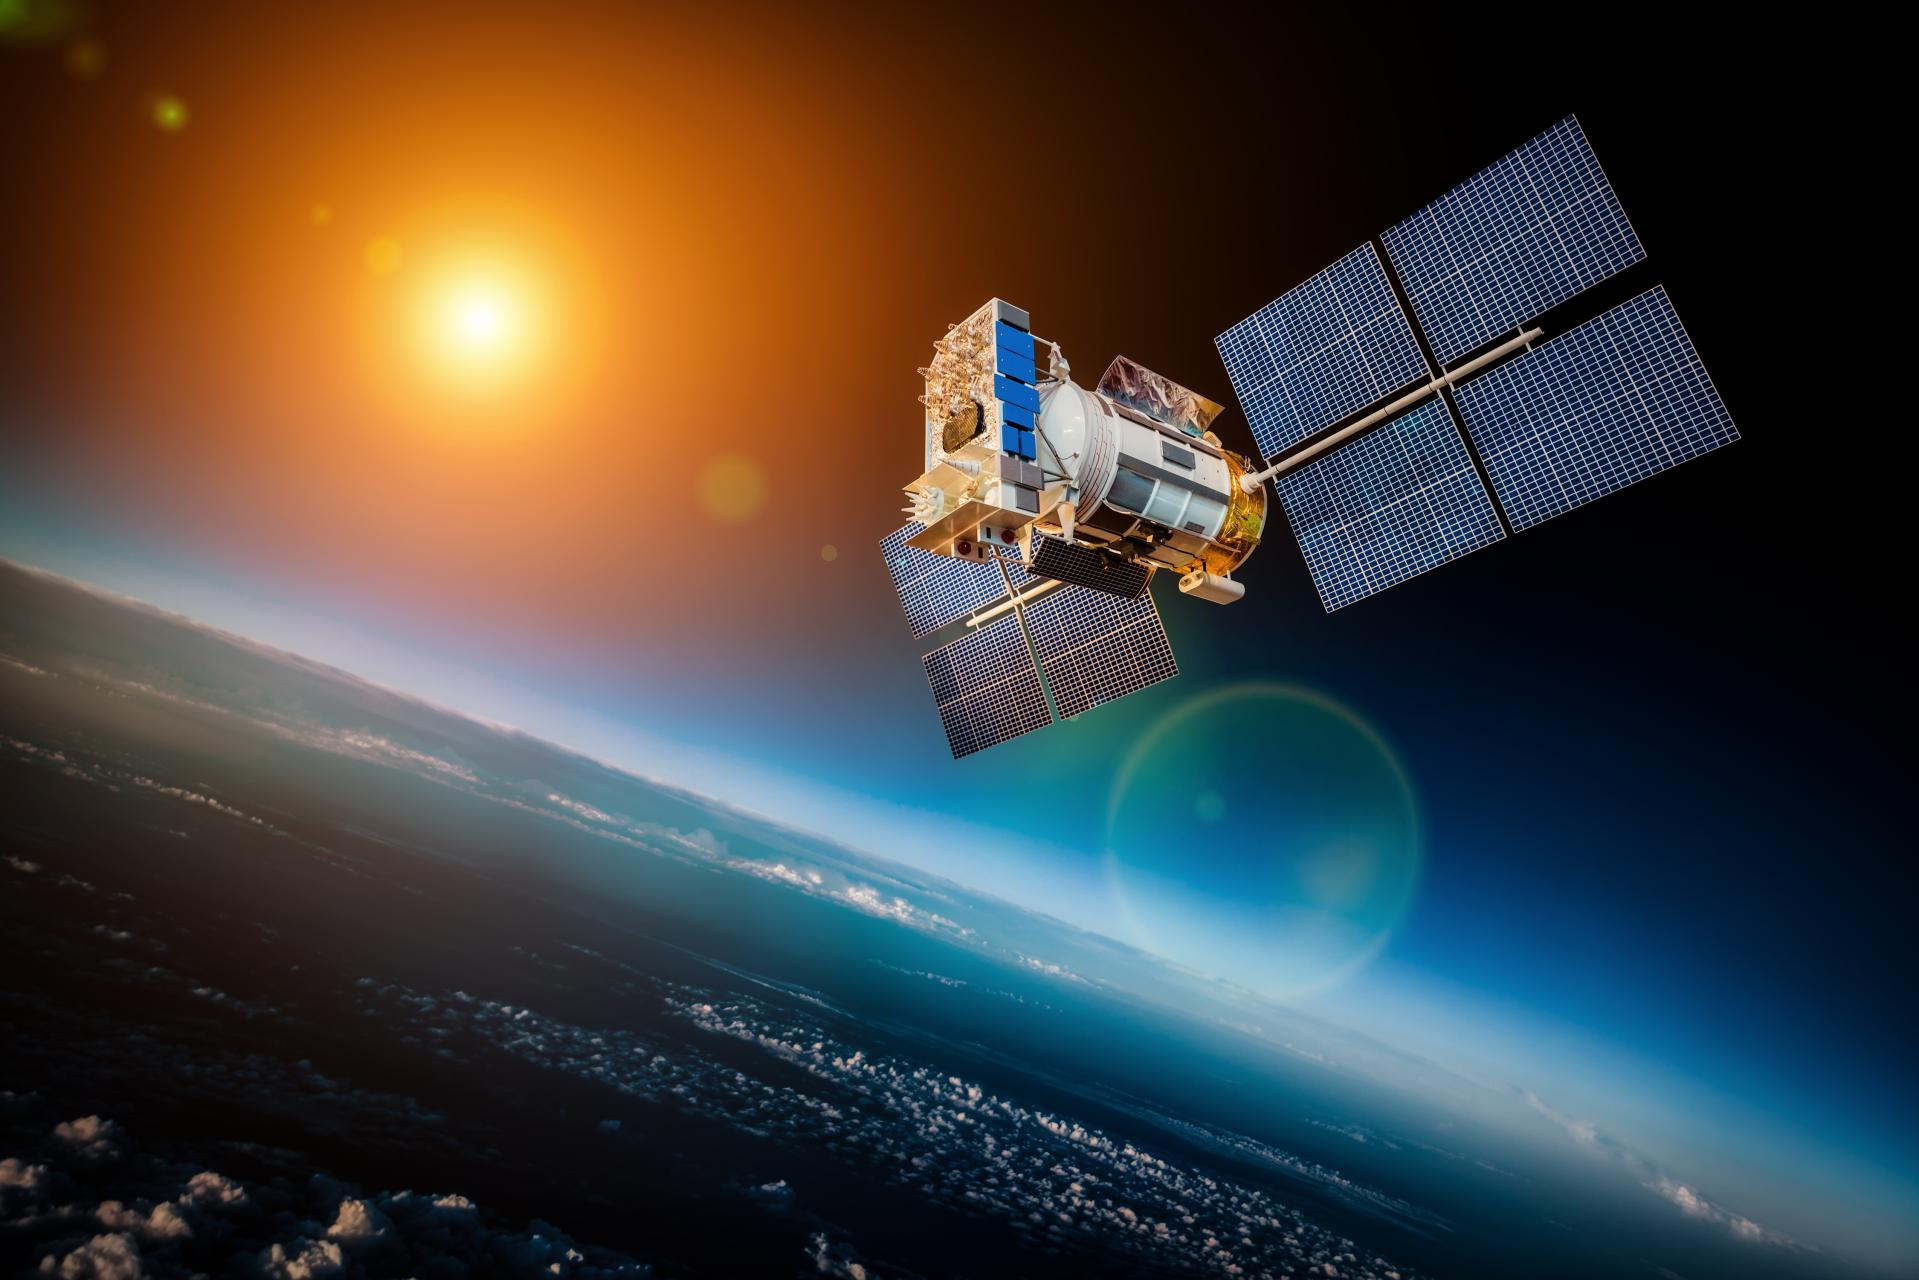
\includegraphics[height = \paperheight, width = \paperwidth]{satellite.jpg}}
    \begin{frame}[plain]\end{frame}
}

\begin{frame}[fragile]
    \frametitle{More slides}

    

\end{frame}

\end{document}